%
%
\subsection{PROCEDURE}
\subsubsection{Planejamento}
Aqui criaremos um procedimento\footnote{Análogo a uma função do tipo \texttt{VOID} (pois procedimentos não retornam valores) numa linguagem de programação, um \texttt{PROCEDURE} ou procedimento é um bloco de código que pode ser armazenado e executado em um banco de dados\cite{Procedure}.} para agendar uma nova consulta, daremos a ele o nome de \texttt{Agendar}.

Para isso, serão necessários cinco parâmetros, são eles: \texttt{id\_paciente}, \texttt{id\_medico}, \texttt{data}, \texttt{hora\_inicio} e \texttt{hora\_fim}.

Dessa forma, o procedimento verificará se já existe alguma consulta marcada com o médico; em caso negativo, a consulta será agendada; em caso positivo, uma mensagem de erro aparecerá para o usuário. Abaixo é possível conferir o fluxograma do nosso procedimento:

\begin{figure}[H]
    \centering
    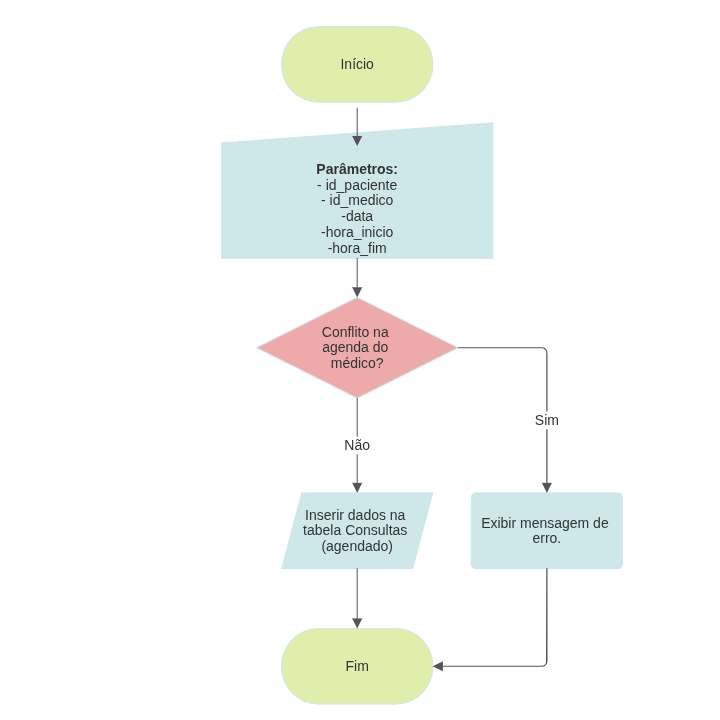
\includegraphics[width=0.75\linewidth]{Text/Proc/flowchart.png}
    \caption{Fluxograma da lógica do procedimento \texttt{Agendar}}
    \label{fig:agendar_flow}
\end{figure}

\newpage
\subsubsection{Execução}

Para declarar um procedimento, primeiro precisamos de um \texttt{DELIMITER}\footnote{Um delimitador (\texttt{DELIMITER}) pode ser entendido como uma notação que marca início e fim de um bloco de código, ele tem prioridade sobre o "\texttt{;}" , isto é, o código não termina com o "\texttt{;}"\ quando está dentro de um delimitador\cite{Delimiter}.}. Com isso começamos o código para nosso procedimento. Vamos dividi-lo em blocos mas é possível vê-lo por completo no Apêndice na subseção \textbf{\ref{subsec:proc} p. \pageref{subsec:proc}}.

\begin{lstlisting}[
    language=MySQL,
    caption=Declaração do procedimento e de variável
]
DELIMITER $$

CREATE PROCEDURE Agendar(
    IN p_id_paciente      INT,
    IN p_id_medico        INT,
    IN p_data_consulta    DATE,
    IN p_hora_inicio      TIME,
    IN p_hora_fim         TIME
)
BEGIN
DECLARE conflito_medico INT DEFAULT 0; 
\end{lstlisting}

Como estamos lidando com inserção de dados precisamos garantir a integridade dos mesmos, assim, usaremos \texttt{TRANSACTION}\footnote{Uma série de comandos \textbf{DML} com mecanismo de segurança de integridade que permitem cancelar toda a operação sem afetar os dados já escrito caso aconteça algum erro\cite{TRANSACTION}.}, logo, se acontecer algum erro durante a execução do procedimento, não há risco dos dados existente serem corrompidos.

\begin{lstlisting}[
    language=MySQl,
    caption=Verificação de conflitos no agendamento
]
-- Inicia a transacao
START TRANSACTION;

-- verifica data e hora sao validas
IF (p_data_consulta < CURDATE()
    OR
    p_data_consulta = CURDATE() AND p_hora_inicio < ADDTIME(CURTIME(), '01:00:00')
   ) THEN

    SIGNAL SQLSTATE '45000'
    SET MESSAGE_TEXT = 'Erro: Hora ou data nao validos!';
END IF;


-- Verifica conflito na agenda do medico
SELECT COUNT(*) INTO conflito_medico
FROM Consultas
WHERE id_medico = p_id_medico
    AND data_consulta = p_data_consulta
    AND status_consulta != 'cancelado' -- Ignora consultas canceladas
    AND ( 
        -- Conflito: nova consulta inicia durante uma existente
        (p_hora_inicio >= hora_inicio AND p_hora_inicio < hora_fim) 
        OR
        -- Conflito: nova consulta termina durante uma existente  
        (p_hora_fim > hora_inicio AND p_hora_fim <= hora_fim) 
        OR
        -- Conflito: nova consulta engloba uma existente
        (p_hora_inicio <= hora_inicio AND p_hora_fim >= hora_fim)
    );    
\end{lstlisting}

Acima temos duas verificações feitas para que o agendamento seja realizado.
\begin{itemize}
    \item \textbf{Linha 5 a 12} - Verifica se as datas são válidas usando funções nativas do MySQL como \texttt{CURDATE()} e \texttt{CURTIME()}, elas retornam a atual do servidor e o horário, respectivamente.
    \item \textbf{linha 16  a 30} - Verifica se o médico tem alguma consulta marcada para o dia e horário desejado. Note na linha 20 que caso a consulta esteja marcada como "\textbf{cancelado}", a verificação a ignora.
\end{itemize}

Finalmente temos:

\begin{lstlisting}[
    language=MySQL,
    caption=Final do código
    ]
-- Na ausencia de conflitos:
IF conflito_medico = 0 THEN
    INSERT INTO Consultas 
        (id_paciente, id_medico, data_consulta, hora_inicio, hora_fim, status_consulta)
    VALUES
        (p_id_paciente, p_id_medico, p_data_consulta, p_hora_inicio, p_hora_fim, 'agendado');

    COMMIT; -- Confirma a transicao
    
    SELECT 'Consulta agendada com sucesso!' AS Mensagem;
    SELECT * FROM Consultas WHERE 
        id_paciente=p_id_paciente AND 
        data_consulta = p_data_consulta AND 
        hora_inicio = p_hora_inicio;
    
ELSE -- Se conflito:
    ROLLBACK; -- Cancela as mudancas na transiction    
    
    SIGNAL SQLSTATE '45000'
    SET MESSAGE_TEXT = 'Erro: Medico ja possui uma consulta agendada nesse horario';
END IF;

END $$
DELIMITER ;
\end{lstlisting}

Aqui, inserimos ou não os dados na tabela. \begin{itemize}
    \item \textbf{Linha 2 a 14} - Caso não exista conflitos, a consulta é agendada com sucesso. Uma mensagem indicando que tudo foi bem sucedido aparece para o usuário juntamente com os dados da consulta agendada.
    \item \textbf{Linha 16 a 20} - Caso contrário, a consulta não é marcada. Uma mensagem de erro aparece para o usuário e a transação é cancelada. Aqui usamos o \texttt{SIGNAL\_STATE '45000'}, onde retornamos um código de erro, no caso, 45000 se refere a um caso genérico retornado pelo usuário\cite{MySQL_45000}.
\end{itemize}

\
\subsubsection{Testando o Procedimento}

Aqui testaremos o funcionamento do procedimento de forma simples. Primeiro vamos ver os dados que temos em Consulta:

\begin{figure}[H]
    \centering
    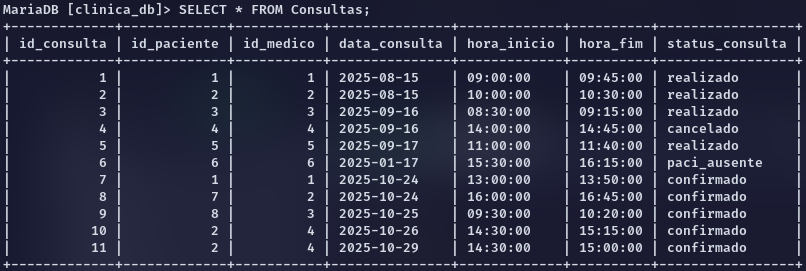
\includegraphics[width=0.8\linewidth]{Text//Proc/select_consulta.png}
    \caption{\texttt{SELECT * FROM Consultas;}}
    \label{fig:select_consulta}
\end{figure}

Agora vamos tentar inserir um dado de tal forma que aconteça um conflito na agenda, logo, usaremos o paciente 2 e o médico 4 para agendar uma consulta no dia 29/10/2025 as 14:50.
Depois vamos tentar inserir uma consulta com o mesmo paciente e médico no mesmo dia, porém as 16:00 horas.

\begin{figure}[H]
    \centering
    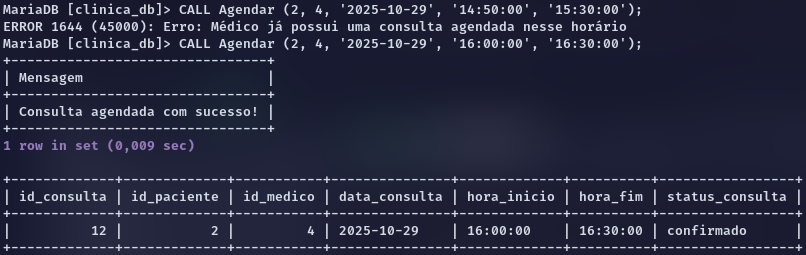
\includegraphics[width=1\linewidth]{Text//Proc/sucesso.png}
    \caption{Note que na primeira tentativa tivemos um erro e após escolher um horário disponível, tivemos sucesso.}
\end{figure}

\begin{alertbox}
    \begin{center}
        \textbf{Nota}
    \end{center}
    O teste aqui realizado não demonstra o completo funcionamento do procedimento, isto é, para todos os casos. Para isso, deveríamos fazer exaustivos testes englobando todas as possibilidades. Entretanto, o objetivo aqui é apenas demonstrativo.
\end{alertbox}

\subsection{Funções}
Nessa subseção trataremos de Funções. Aqui criaremos uma função simples, ela receberá um parâmetro que é o ano de nascimento de um paciente do tipo \texttt{DATE}, calculará com base na data do servidor sua idade, retornando assim, um valor inteiro.

Veja o código a seguir:

\begin{lstlisting}[
    language=MySQl,
    caption=Função Calc\_idade
]
DELIMITER $$

CREATE FUNCTION Calc_Idade (
    f_data_nascimento DATE
)

RETURNS INT
DETERMINISTIC

BEGIN 
    DECLARE idade INT;
    SET idade = TIMESTAMPDIFF(YEAR, f_data_nascimento, CURDATE());
    RETURN idade;
END; $$

DELIMITER ;
\end{lstlisting}

\begin{itemize}
    \item \textbf{Linha 3 a 8} - Aqui definimos a função, ela recebe um parâmetro \texttt{f\_data\_nascimento} do tipo \texttt{DATE}, e retornará um valor \texttt{INT}. Aqui também definimos a função como \texttt{DETERMINIST}\footnote{Uma função é dita determinista se, dadas as mesmas condições iniciais, isto é, os mesmos valores nos parâmetros, ela retornará o mesmo valor\cite{MySQL_deterministic}.}
    \item \textbf{Linha 11 a 13} - Aqui fazemos o cálculo da idade usando uma função nativa chamada \texttt{TIMESTAMPDIFF(Unidade, date\_time\_expr1, date\_time\_expr2)}, essa função retorna a diferença entre as datas inseridas. Veja a representação pictórica da função abaixo:

    \begin{figure}[H]
        \centering
        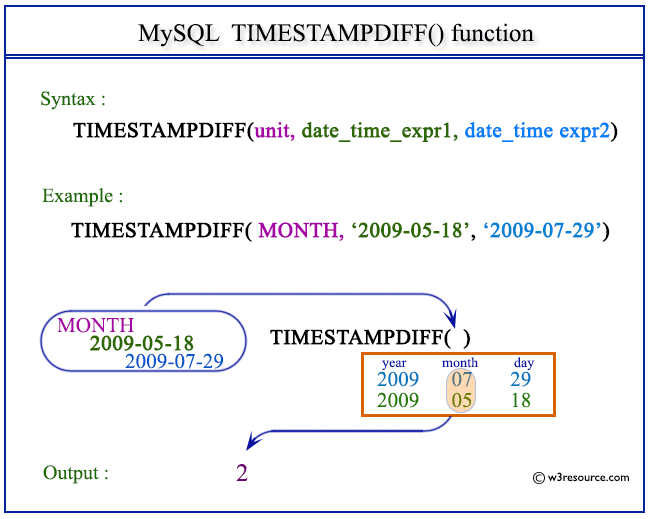
\includegraphics[width=0.75\linewidth]{Text//Proc/TIMESTAMPDIFF.png}
        \caption{Representação Pictórica de TIMESTAMPDIFF\cite{timestamp}}
        \label{fig:placeholder}
    \end{figure}
\end{itemize}

\subsubsection{Testando a Função com VIEW}
Vamos agora testar a função, primeiramente vamos analisar a idade de um paciente isolado, escolheremos o paciente de ID 3. Assim, com o comando \texttt{SELECT Calc\_Idade(data\_nasc) FROM Pacientes WHERE id\_paciente = 3;} temos:

\begin{figure}[H]
    \centering
    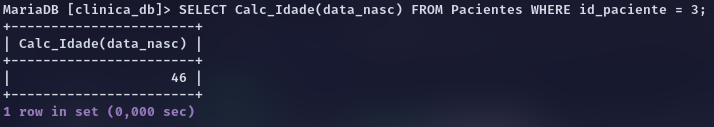
\includegraphics[width=1\linewidth]{Text//Proc/idade_3.png}
    \caption{\texttt{SELECT Calc\_Idade(data\_nasc) FROM Pacientes WHERE id\_paciente=3;}}
    \label{fig:placeholder}
\end{figure}

Agora, vamos usar a função para ver a idade de todos os pacientes. Como essa pode ser uma consulta usual, é interessante criarmos uma \texttt{VIEW}. Para isso usamos o comando a seguir:

\begin{lstlisting}[
    language=MySQL,
    caption=Criando \texttt{VIEW v\_paciente\_idade}
]
CREATE VIEW v_pacientes_idade AS
SELECT 
    id_paciente,
    nome,
    data_nasc,
    Calc_Idade(data_nasc) AS idade
FROM Pacientes;    
\end{lstlisting}

Assim, com um simples \texttt{SELECT * FROM v\_pacientes\_idade;}:

\begin{figure}[H]
    \centering
    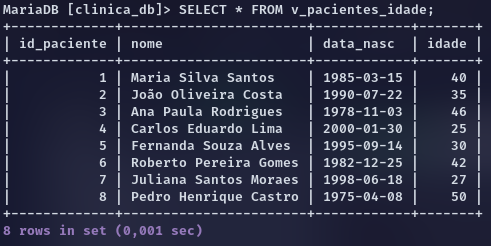
\includegraphics[width=0.75\linewidth]{Text//Proc/idade_table.png}
    \caption{\textbf{\texttt{SELECT * FROM v\_pacientes\_idade;}}}
\end{figure}

 Vamos aproveitar e criar um \texttt{VIEW} mais complexo onde podemos aplicar a função. Queremos agora um \textit{output} de todos os pacientes que tem consultas marcadas nos últimos 15 dias, e em vez de mostrarmos a data de nascimento, vamos pedir apenas a idade.

\begin{lstlisting}[
    language=MySQL,
    caption=Criando \texttt{VIEW v\_paciente\_agendados\_15}
]
CREATE VIEW v_pacientes_agendados_15 AS
SELECT 
    p.id_paciente,
    p.nome,
    Calc_Idade(data_nasc) AS 'Idade',
    c.data_consulta AS 'Data Consulta',
    c.status_consulta AS 'Status Consulta'
FROM Pacientes AS p
JOIN Consultas AS c
    ON p.id_paciente = c.id_paciente
WHERE
    TIMESTAMPDIFF(DAY, c.data_consulta, CURDATE()) <= 15;
\end{lstlisting}

Assim:

\begin{figure}[H]
    \centering
    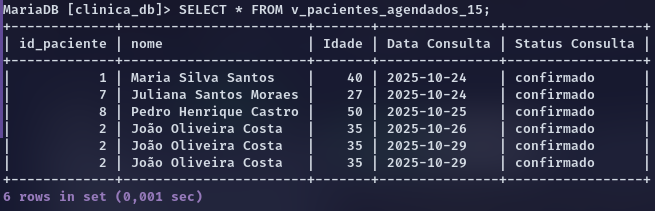
\includegraphics[width=1\linewidth]{Text//Proc/image.png}
    \caption{\texttt{VIEW v\_pacientes\_agendados\_15}}
\end{figure}

